\documentclass[12pt,openany]{book}

%PACKAGES%
\usepackage[inner=25.86mm, outer=18.24mm, top=25.86mm, bottom=33.48mm, papersize={154mm, 216mm}]{geometry}
\usepackage{graphicx}
\usepackage{fontspec}
\usepackage{enumitem}
\usepackage{sectsty}
\usepackage[]{titlesec}
\usepackage{verse}
\usepackage{fix-cm}%font size
\usepackage{multirow}%tables
\usepackage{array}%tables
\usepackage[hyphens]{url}
\usepackage[toctextentriesindented]{tocstyle}
\usepackage{tocloft}
\usepackage{soulutf8}
\usepackage{marginnote}
\renewcommand*{\marginfont}{\SkolarLight}

%this snippet of code is a bit of a hack to allow line break after em-dash (http://tex.stackexchange.com/questions/62800/lualatex-and-line-breaks-after-em-dashes)
\catcode`\—=13
\protected\def—{\unskip\textemdash\allowbreak}

%\usepackage{pagegrid}
%PACKAGES%
%\pagegridsetup{top-left, step=3.435in}

%TABLE OF CONTENTS%
\settocstylefeature[]{leaders}{\hfill}%ELIMINATES DOTS%
\settocstylefeature[0]{entryvskip}{0.5em}%VERTICAL SPA\caps{ce} BEFORE CHAPTER ENTRIES%
\renewcommand*{\cfttoctitlefont}{\Secfont\Large}%use tocloft
%TABLE OF CONTENTS%

%LINESPACE% SETS LINESPA\caps{ce}
\usepackage{setspace}
\setstretch{1.15}
%LINESPACE%

%FONTS% These are the normal SC fonts. We have a ``light'' skolar, too. 
\setmainfont[Numbers=OldStyle]{Alegreya ht Pro}
\setsansfont[Scale = MatchLowercase]{Source Sans Pro}
\setmonofont{Source Code Pro}
% \newfontfamily\SkolarLight{Alegreya Sans SC Light}

\newfontfamily\Chapfont[ItalicFont=Alegreya Sans Italic]{Alegreya Sans}
\chapterfont{\Chapfont\LARGE\centering\mdseries\setstretch{1}}
\newfontfamily\Secfont[Numbers=OldStyle]{Alegreya Sans Medium}
\sectionfont{\Secfont\mdseries\large\setstretch{1}}


%HEADINGS%

%HEADER% 
\usepackage{fancyhdr, textcase}
\setlength{\headheight}{15pt}
\pagestyle{fancy}
\renewcommand{\chaptermark}[1]{\markboth{\thechapter.\ #1}{}}
\renewcommand{\sectionmark}[1]{\markright{\thesection\ #1}}

\fancyhf{}
\fancyhead[LE,RO]{\thepage}
\fancyhead[CO]{\headcaps{\MakeUppercase{Ajahn Brahmali}}}
\renewcommand{\headrulewidth}{0pt}
\fancypagestyle{plain}{ %
\fancyhf{} % remove everything
\renewcommand{\headrulewidth}{0pt}
\renewcommand{\footrulewidth}{0pt}}
\newfontfamily\headcapsfont[RawFeature=+c2sc]{Alegreya ht Pro}
\newcommand\headcaps[1]{{\headcapsfont #1}}
\fancyhead[CE]{\headcaps{\MakeUppercase{Samatha \& Vipassanā}}}
%HEADER%

%HANGING LEFT%
\newcommand*{\vleftofline}[1]{\leavevmode\llap{#1}}
%HANGINGLEFT%

%WIDOWS & ORPHANS% 
\widowpenalty=10000
\clubpenalty=10000
%WIDOWS & ORPHANS%

%Applies various subtle improvements in typography. Use default.
\usepackage{microtype}
\frenchspacing

\usepackage[unicode, hidelinks, pdfauthor={Brahmali}, pdftitle={Why Samatha and Vipassanā are Inseparable}, pdfsubject={Buddhism}, pdfkeywords={Buddhism, bhikkhu, monks, Sutta, tipitaka, tripitaka, sutra, samatha, vipassana, calm, insight}, pdfproducer={LuaTeX  beta-0.70.1}, pdfcreator={LaTeX2e}]{hyperref}

%DOCUMENT INFO. NOT USED IN TEXT.%
\title{Why Samatha and Vipassanā are \protect\\ Inseparable}
\author{Ajahn Brahmali}
\date{}
\begin{document}
\frontmatter
\pagestyle{empty}
\newgeometry{margin=0px}

\hspace*{-156mm}
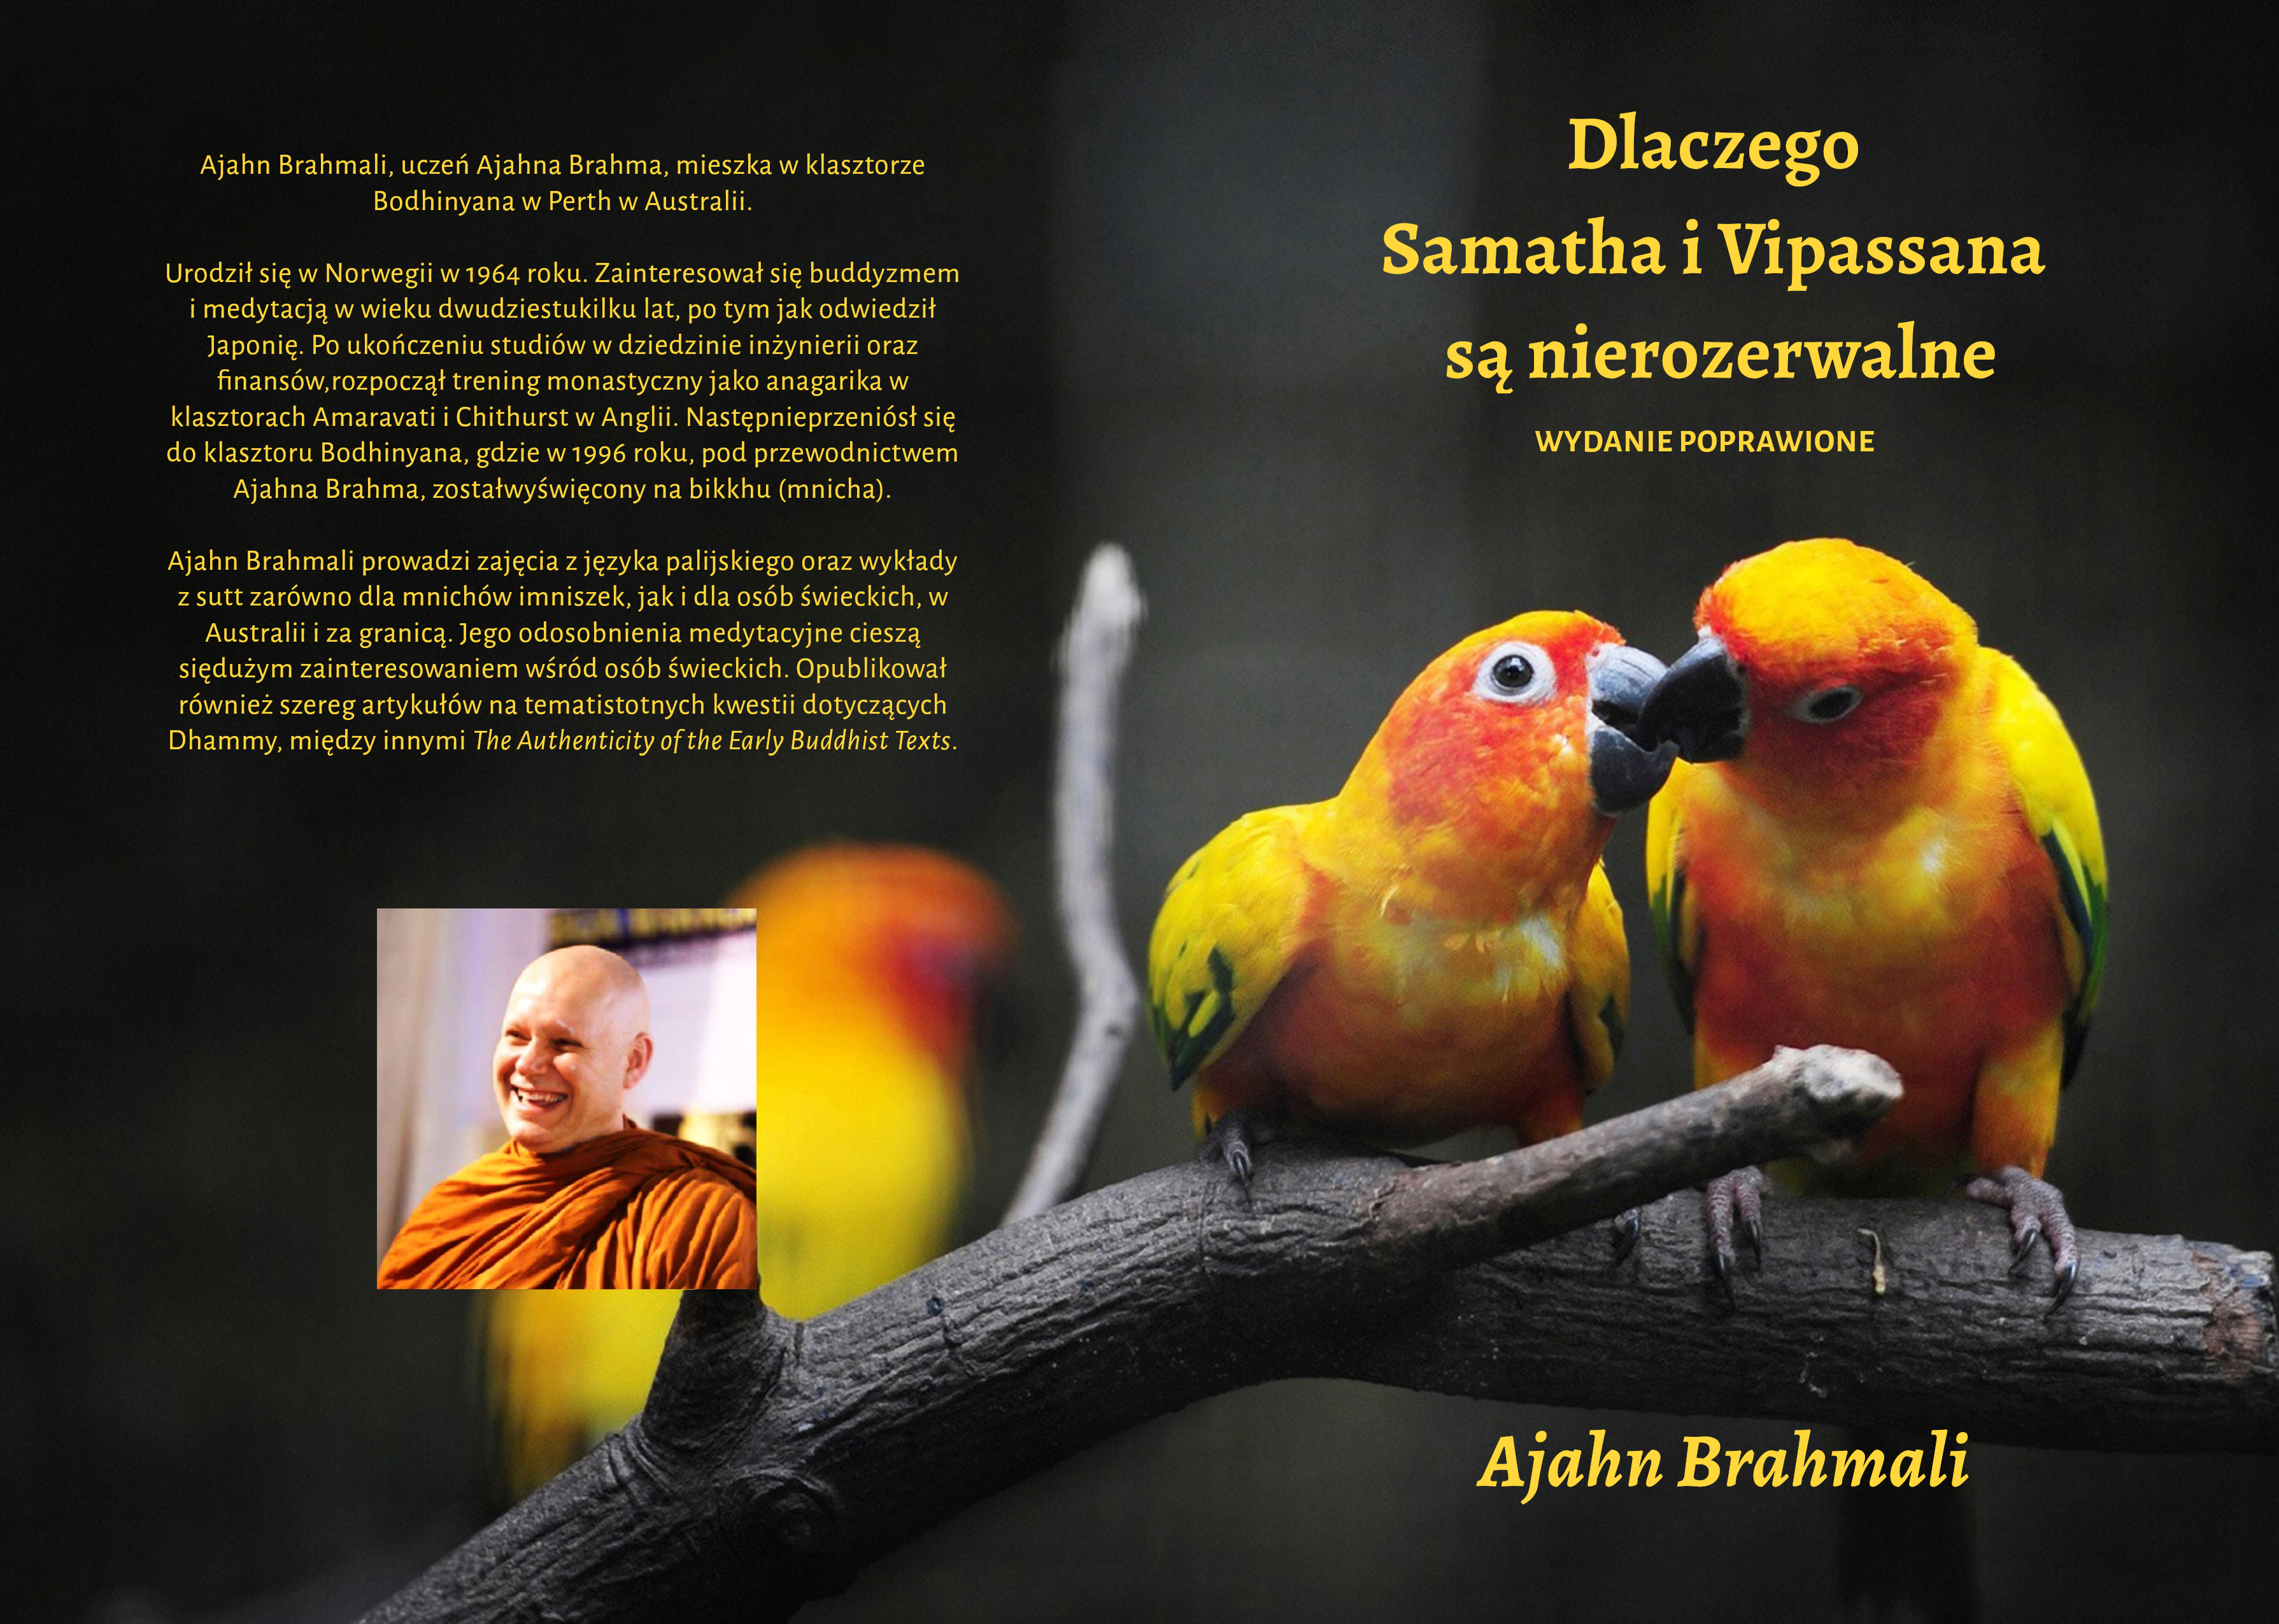
\includegraphics{sv-2_a5_cover}

\begin{center}\end{center}
\begin{center}

\vfill

\maketitle

\vfill
\end{center}

\newpage
\restoregeometry

\begin{center}\end{center}

\vspace{4em}
{\small
\noindent Based on a talk given on Friday 8th of May, 2015 \\at Dhammaloka Buddhist Centre, Perth, Australia.

\bigskip

\noindent Copyright Ajahn Brahmali.
\bigskip

\noindent Compiled and Published by:

\medskip

\noindent Ajahn Brahm Society of Sri Lanka

\noindent 380/9, Sarana Road, Colombo 7, Sri Lanka

\noindent abs.sl.list@gmail.com

}

\vfill

\begin{center}
\textit{May all beings be well and happy!}

\end{center}
\vfill

\newpage

\begin{center}\end{center}
\begin{center}

\vfill

{\huge \textit{Why} 

\medskip

\textbf{Samatha} \textit{and} \textbf{Vipassanā} 

\bigskip

\textit{are Inseparable}}

\vfill

\caps{\LARGE Ajahn Brahmali}

\vfill
\end{center}

 \newpage

\begin{center}\end{center}
\begin{center}

\vfill

\textit{\large I am at a loss for words when people ask me: \\“Do you teach vipassanā meditation?”}

\vfill

\end{center}

\newpage
\mainmatter
\chapter*{Introduction}

Quite regularly people call our monastery in Perth to inquire whether we teach \textit{vipassanā} meditation. I am at a loss when people ask that question, and so I say, “Yeah, in one way we teach \textit{vipassanā} meditation, but in another way perhaps not.” Or I say, “We teach Buddhist meditation,” or something to that effect. I don’t want to make things too complicated or controversial when someone is new to the Dhamma and meditation practice.

The ideas of \textit{samatha} and \textit{vipassanā} are central to Buddhist meditation practice. \textit{Samatha} is usually translated as calm, peace, or tranquillity, while \textit{vipassanā} is normally translated as insight. In the course of this text I intend to discuss how appropriate these renderings are. To do this we need to understand how these words were used by the Buddha.

\chapter*{The problem with “\textit{vipassanā} meditation”}

\pagestyle{fancy}

In the \textit{suttas}, the Buddha talks about \textit{vipassanā} and he talks about meditation, but he never joins the two terms together into “\textit{vipassanā} meditation”. Despite the common contemporary use of this phrase, the fact is that the Buddha never used it. What, then, is \textit{vipassanā}? And what is its connection to \textit{samatha}? These are main issues that I discuss in this essay.

It’s easy to understand why people are interested when they hear about \textit{vipassanā} meditation. It sounds attractive and powerful. Who doesn’t want insight? Insight means wisdom, it means understanding, it means having clarity about things. It means knowing your body and mind, understanding your personal universe, and having insight into its nature. Wisdom is the most important mental faculty for personal meaning and happiness. When I hear the phrase “insight meditation”, my initial response is, “Wow, a meditation that leads to wisdom; that’s exactly what I want.” Insight meditation is a powerful phrase and that is likely to be a key reason why it has taken off. Yet the Buddha never used it.

There are good reasons why the Buddha never spoke of \textit{vipassanā} meditation. One of the consequences of using this expression is that you separate \textit{samatha} from \textit{vipassanā}. By speaking of insight meditation, you are implying there is something else called calm meditation. But the Buddha didn't use the phrase “calm meditation”, either. In the \textit{suttas}, rather, \textit{samatha} and \textit{vipassanā}, calm and insight, are outcomes of the practice, not practices in their own right. And they are normally conjoined, constituting two aspects of the same process of mental development.

Moreover, once you have established the idea of insight meditation and you emphasise it and give it pre-eminence, you imply that other meditations, specifically calm meditation, is less important. The very fact that you emphasise one implies something about the other, even if this is not explicitly stated. This is another reason why I think it is unfortunate to talk about insight meditation: it is an implied value judgement about what matters on the Buddhist path.

\chapter*{\textit{Samatha} and \textit{vipassanā}: what they really mean}

Before we discuss the process of meditation in more detail, we need greater clarity about what \textit{samatha} and \textit{vipassanā} really refer to.

\section*{\textit{Samatha}}

What \textit{samatha} means is generally uncontroversial. It is used throughout the \textit{suttas} and the \textit{vinaya} in an unambiguous way to refer to calm or tranquillity, whether externally in the community or internally in one’s own private experience. Anyone who has meditated will have some idea of what this private experience is like. When you sit down and close your eyes and your meditation goes well, you feel calmer afterwards. What does this mean? It means your mind is less restless. It means there are fewer desires and defilements in the mind. It means you feel more relaxed and at ease. It is a very positive experience. A feeling of calm is preferable to feelings of agitation, restlessness, and desire.

The interesting thing is that the little bit of calm you feel after a nice meditation is only the beginning of this beautiful journey in Buddhism. The degree of calm increases, stage by stage, until you feel a sense of peace and calm that would previously have been unimaginable. There is a profundity to this calm. As you experience this, you begin to understand why meditation is so special, to the point where it gets you in touch with the very meaning of life. Gradually everything becomes incredibly peaceful and still. Your normal world disappears and you see everything in an entirely new light.

So calm is a relative thing. You may think you are calm after meditating, but then you become even calmer. Looking back on the previous meditation you think, “Hey, that was not calm at all; that was restless!” Then you become calmer still and again you think back on the previous level, “That wasn’t very calm either.” As you continue in this way, stage by stage, you start to get a proper perspective on life. The more peaceful you are, the more you understand what suffering is and what life is all about. Being truly calm is both transformative and blissful. Eventually you take that to a very profound level.

This is \textit{samatha}.

\section*{\textit{Vipassanā}}

The other side of this \textit{samatha}\textit{-vipassanā} pair is \textit{vipassanā}, often translated as insight. To start with, we need to decide how appropriate this translation is. Having studied the word of the Buddha in quite a bit of detail, I think this rendering can be improved upon.

From a linguistic point of view, \textit{vipassanā} is composed of the prefix \textit{vi-} plus the word \textit{passanā}, which means “seeing”. So we are dealing with a particular kind of seeing, the precise kind being determined by the function of the \textit{vi-}. Now the prefix \textit{vi-} is used to convey a number of different meanings, two of which are most relevant for the present context. One of these is the idea of separation. In this sense \textit{vi-} denotes discrimination or analysis, and \textit{vipassanā} might then be translated as analytical seeing or insight. But \textit{vi-} is also used to denote intensification, which might lead us to render \textit{vipassanā} as “really seeing” or “clear seeing”. So which one of these is correct?

There is one \textit{sutta} in particular that sheds light on this. In this \textit{sutta}, AN 2.31, \textit{vipassanā} is said to lead to \textit{paññā}, wisdom. If we render \textit{vipassanā} as insight, we must understand this \textit{sutta} as saying that insight leads to wisdom. Yet in English the two words insight and wisdom are barely distinguishable, especially in a spiritual context. If \textit{vipassanā} leads to wisdom, we require a rendering of \textit{vipassanā} that does not denote wisdom itself, but instead a stepping-stone towards it. Given the two options available from our linguistic analysis above, clear seeing is therefore preferable to insight.

But there is more. According to the Mahāpadāna Sutta (DN 14) there was a previous Buddha called Vipassī, a name that means “one who has \textit{vipassanā}”. The same \textit{sutta} states that he received his name because past \textit{kamma} had made him clairvoyant from birth and because he was “unblinkingly watchful, like the gods of the Thirty-Three”. Both of these reasons support the rendering of \textit{vipassanā} as clear seeing, but not as insight.

Now, there is an important difference in English between insight and clear seeing. Insight refers to something that happens instantly, “Wow, now I understand!” It is a moment of realisation, a flash of lightning in the mind’s eye. This metaphor is actually found in the \textit{suttas} to illustrate steamentry, a profound moment of insight. Clear seeing, by contrast, is something that is always either present or absent, in varying degrees. Right now you either see things clearly or you don't, or you are somewhere in between. If you imagine clear seeing as a sliding scale that starts at utter confusion and ends with full clarity of mind, then you are always at some point on that scale.

So in a meditation context your \textit{vipassanā} gradually increases as your meditation improves. Just as you are \textit{calmer} after a good meditation, you also have more \textit{vipassanā}. When you then look inside of yourself, it is easier to see the state of your mind. Instead of your mind just rushing along from one idea to another, or from one mental state to another, you now have enough clarity to see what is there. You see things arise and you see them pass away. You see the defilements—their arising, their presence and their disappearing. From a meditation perspective this is what \textit{vipassanā} is about: the ability to clearly see what is happening, especially what is going on inside of you.

This sort of clear seeing is a critical part of the spiritual path. The more awareness you have of what is going on in your mind, the greater is your ability to do something about it. Clear seeing is the necessary foundation that enables you to change your perceptions and the way you think. It allows you to guide your life in a new direction, towards wholesome qualities, towards that which create happiness in life rather than suffering. And as you progress on the path, the clear seeing becomes more and more refined. The deeper the calm of the meditation, the more clearly you see and the greater is your ability to steer your mind in the right direction.

Not only do you see the defilements but you also see how they arise from causes. This idea of causality is so important in Buddhism. Why is it that you think in a certain way? Why is it that you perceive in a certain way? As clear seeing deepens, you see how things are built up of chains of causality, one thing leading to the next. The mind moves according to cause and effect. When you understand the structure of your experience, how causes and results follow each other, you can start to change the content of your mind. Change the conditions and you get different results. This is the point of understanding causality, and it is an essential part of \textit{vipassanā}. You understand the defilements of the mind and the good qualities of the mind, and you understand how they come about.

Let me give a practical example. When you do \textit{mettā} meditation, you may sit down and say, “May all beings be happy and well.” In this case it is quite obvious why the beautiful feeling of \textit{mettā} arises. You see from your own experience that it arises because you are focusing on the goodness and the positive qualities in yourself and other people.

Just like \textit{samatha}, \textit{vipassanā} can be very powerful. It can be taken to great depths on the path of meditation. You can have incredible clarity and see what is happening inside of you in minute detail. And just like \textit{samatha}, \textit{vipassanā} is a relative concept. Stage by stage it becomes more and more powerful, until it reaches the highest levels.

So \textit{samatha} and \textit{vipassanā} refer respectively to calm and clear seeing. They are both results of the practice, not something you do. But if the Dhamma is all about causality, then how, exactly, do these two qualities come about?

\chapter*{What prevents and what causes clear seeing}

Let us consider \textit{vipassanā} first. If there is no such thing as \textit{vipassanā} meditation in the \textit{suttas}, what is it that gives rise to clear seeing?

It will probably come as no great surprise that the answer is \textit{sīla}, which for present purposes can be rendered as purity. So the purer you are and the purer your mind is, the greater is your ability to see things clearly and in accordance with reality. But why is it that a lack of defilements and the presence of wholesome qualities give rise to clear seeing? How does this work?

\section*{Desire}

If you look carefully, you will notice that whenever you desire something, and especially if you are attached to it, you have a vested interest in that thing. You are looking at it from certain perspective, looking for its attractive features. But seeking out specific aspects of something is by definition a bias. And bias is the opposite of clear seeing. It is not detached, and it involves a distortion in outlook. You are not just standing back and watching things as they actually are.

Why does craving arise in the first place? Why is it that we have certain inclinations that make us crave for certain things? Very often it is because of our habits and views, the way we have been conditioned to look at the world. Some of our habits and views are formed in childhood. We were brought up in a certain way, in a certain culture, and we have acquired corresponding habits. But for the most part our habits come from past lives. Consequently it is often useless to try to understand where our habits and views come from.

I will give a trivial example of what I mean by habits. I was born in Norway. If you were born in Norway, you tend to like certain foods. Some of the foods I think are great would probably be disgusting to you. You might wonder how anyone could eat such food. This is cultural conditioning. This kind of conditioning is very obvious in our monastery. People born in Sri Lanka normally bring dhal, whereas people with a Chinese background often bring Chinese food. All the various groups of people who visit us act in a similar fashion.

So we are conditioned by our backgrounds. What we like in this world and what we crave for is conditioned. We have certain habits and views about things and that leads to particular cravings. We are thoroughly biased about the things of the world. There is no clear seeing.

It is astonishing how powerful these biases can be. Consider our views about the world. Often we have strong political persuasions—towards the left, towards the right, somewhere in the middle, or whatever—and we are absolutely sure our way of looking at the world is right. If someone disagrees with us, they are wrong. If you didn’t think that, you wouldn’t have that view.

When you look at it from a Buddhist perspective however—whether it’s a political view, a religious view, or any view—they are all conditioned. It all comes from the past. We think we are rational beings, that we see things our way because we are sensible, but most of the time it’s just a matter of conditioning.

Sometimes a person’s view flips over. They are on one side of the political spectrum and after a few years they are on the opposite side. “I was wrong before, now I’m right!” Or you go from one religion to another. Or you go from not believing in rebirth to believing in it. I have seen this with so many people. They say, “Rebirth is nonsense; it’s irrational.” But after a few years they change their mind. Suddenly rebirth is acceptable. So which view was the rational one? Probably neither of them, because most likely they were both conditioned into existence. (This is to say nothing about the truth of a view, only how it arises.) It is conditioning that makes any particular view prominent. When you see that, you don’t take your views so seriously and you become more flexible in your outlook.

So the point here is that craving is a problem, because craving is inherently biased. When you crave, you start acquiring—relationships, friendships, possessions, status. As a consequence you attach. Attachments, too, are a form of bias. If you have children, for instance, you care about how they behave. People often get upset if their child behaves badly in front of others. You feel upset because you feel they reflect something about you, as if they are an extension of your personality. And because you have a vested interest in how they behave, you are biased. So the defilements of the mind, especially desires and attachments, give you a particular inclination. Because they bend your outlook, there is no way you can see things clearly.

What are the implications of this? It means that \textit{vipassanā} is impossible in such circumstances. It shows you why purity of mind is so important for clear seeing.

\section*{Anger}

It is exactly the same with anger. When you are angry you think, “I've got to tell them off; I've got to give them a piece of my mind,” but afterwards you often regret it. You realise that the anger distorted your thinking, that it led you astray. You did something that you wouldn’t have done if your mind had been clearer. And as a consequence you often regret your actions afterwards.

\section*{Purity}

So this is why \textit{vipassanā}, clear seeing, only happens with a pure mind. As you reduce the defilements of the mind, the beautiful qualities of the mind emerge by themselves—the kindness, the compassion, the generosity—and the more clarity you have. You start seeing the world more in accordance with reality.

Purity of mind is what drives \textit{vipassanā}. This means that \textit{sīla} is a critical factor on the Buddhist path. It is only by reducing the defilements and building up good qualities that \textit{vipassanā} comes about.

\chapter*{What prevents and what causes calm}

Now if you look at the other side of the coin, at \textit{samatha}, you realise that that, too, comes from purity. What is it that takes you away from peace and tranquillity? It is often desire. When you desire something, your mind is preoccupied with how to fulfil that desire. You plan and fantasise, thinking about a desired future fulfilment. Or you might be upset about something. You endlessly ruminate over a perceived ill-treatment or injustice from the past. In either case your mind roams around, restless and agitated. This is the opposite of calm.

As you purify yourself of these defilements, the mind is less distracted and it tends to settle down in the present moment. It calms down. In other words, purity is the cause of \textit{samatha}. From this we must conclude that \textit{samatha} and \textit{vipassanā} have the same source.

\chapter*{The source of \textit{samatha} and \textit{vipassanā}}

This result is very interesting because it matches with what we find in the \textit{suttas}. In the discourses of the Buddha, \textit{samatha} and \textit{vipassanā} often appear together, either joined together by the word \textit{ca}, “and”, or conjoined into a single word, a so-called compound. Moreover, the two are often said to develop together as a pair. Now you can appreciate why: it is because they originate from the same source. This means that as you improve your purity and good qualities, it is unavoidable that \textit{samatha} and \textit{vipassanā} develop together. That simple understanding has very important consequences.

The first consequence is that we need to stop thinking in terms of \textit{samatha} meditation and \textit{vipassanā} meditation. Any meditation that gives rise to one of these qualities must also give rise to the other. So if we are getting both calm and clear seeing, we know we are on the right track. If we get none of them, we need to adjust what we are doing. If it seems we are getting one but not the other, it is likely we are actually getting neither. Again, we need to adjust our practice. Moreover, \textit{any} method of meditation—regardless of its label—that gives rise to both qualities is part of the Buddhist path. There is only one proviso: it needs to be supported by right view.

The second and perhaps most important consequence is that we recognise that we should place a strong emphasis on goodness in our lives. We need to regularly contemplate how we can reduce our mental defilements and how we can increase our good qualities. As we put this into practice, \textit{samatha} and \textit{vipassanā} arise together.

So how do we become more pure so that \textit{samatha} and \textit{vipassanā} are strengthened? The obvious starting-point is just kindness, gentleness, and virtue, not forgetting the mental aspect of these things. Do what is good and avoid what is bad. Develop a bit of loving kindness and compassion. Remember that \textit{sīla} is the foundation for any kind of meditation practice, any kind of Buddhist practice. We see this again and again in the \textit{suttas}. The more clear you are about this, the more priority you will give it in your life. Only when you fully integrate all aspects of \textit{sīla} into your everyday life, will it become a force that lifts your meditation, taking \textit{samatha} and \textit{vipassanā} to new heights. When purity is developed with full commitment and perseverance, there is really no limit to how far you can go on the Buddhist path.

\section*{Get inspired by stories of kindness}

Sometimes I hear marvellous stories of kindness within our Buddhist community, and sometimes among non-Buddhists as well. It is important to tell these stories, because when you hear stories of true kindness it uplifts you, inspires you, and pushes you in the right direction. So please tell each other stories about kindness. And don’t tell each other the typical stories you hear on the news—about wars or murders, or whatever bad that humanity gets up to—because that often just drags you down. We need to focus on the good in life. When we do, we realise there is a lot of goodness in our world.

Here is a beautiful story of kindness that I heard recently. A Thai lady who comes to our monastery quite regularly had parked her car outside a Hungry Jack’s restaurant in one of the suburbs of Perth while doing some errands. When she returned to her car, she saw some kids playing and fighting around her vehicle. They were running around the car and some of them were hiding underneath. Because they were hiding under the vehicle, she couldn’t go anywhere. She was stuck. It is all too common in such situations to get upset and tell the kids off for their bad behaviour. It is easy to think of how busy you are and that you don't have the time for this kind of nonsense. But when you realise the importance of kindness in your life, you are always on the lookout for how to respond to any situation in a good way. Because this lady is very good-hearted, she realised this was an opportunity to do good. Inspiration came to her. She said to the kids, “Come on, kids, stop the fighting. Let’s go to Hungry Jack’s for a burger and a drink.” The kids stopped fighting. She then did as promised and everyone was all smiles.

When I heard that story I thought, “Wow, how wonderful it is that we have such people in our community.” But the truth is that these sorts of things happen all the time; we just don't hear about them. Whether it’s in Perth, other parts of Australia, or anywhere else in the world, there are a lot of good-hearted people in our midst. Sometimes all you have to do is to focus on that kindness and it lifts you up. It certainly made me feel happy when I heard that story. What a wonderful thing it is that people do such things!

Another story I heard recently concerns one of the monks in our monastery. This monk had been trying to get his passport renewed. He was going back and forth to the post office and for some reason he was having a very hard time getting his passport done. Eventually everything seemed to be OK, but when he gave the fellow behind the counter a cheque to pay for it all, he was told, “Sorry, we don’t accept cheques.” He was stuck once more. That’s when something remarkable happened. The man behind the counter—just an ordinary Australian, not a Buddhist, and quite likely he had no understanding of Buddhist teachings—he said, “I will pay for you with my own money. You can reimburse me later.” It amounted to over \$250! He didn’t know whether he would ever see this monk again. From his point of view it was little different from just giving the money away. What a wonderful thing to do. And, of course, he did get his money back. Buddhist monks are usually reliable!

As a Buddhist monk I find myself at the receiving end of much kindness, not just from the Buddhist community but from the rest of society as well. When I occasionally go to the shops to buy building materials for the monastery, people sometimes say, “Oh, you are a Buddhist monk. There is no charge for the monastery.” Or they might say, “You only have to pay half the price, because it's for the monastery.” These are the sorts of things I hear quite regularly. And it is always uplifting to know that there is so much kindness and generosity in our world.

When we hear such stories, it helps us do better in our own lives. We feel inspired by the example of others. Then, when we go out of our way to support the people around us, we take society and ourselves forward at the same time. Not only do we create happiness for everyone around us, but we generate so much purity and happiness for ourselves.

As we fill our lives with these kinds of actions—virtue, kindness, compassion, understanding, generosity—we are sure to make real progress on the Buddhist path, especially in \textit{samatha} and \textit{vipassanā}.

\section*{A golden rule for meditation}

Meditation, at least initially, should serve a similar purpose. If we want \textit{samatha} and \textit{vipassanā} to arise, we should meditate to reduce the defilements and the hindrances, and to give rise to positive qualities instead. Meditation practice becomes a continuation of the purification process that started with the earlier factors of the noble eightfold path. Once you are clear about this, you know how to monitor your progress. If your meditation is helping you to reduce your unwholesome qualities and to give rise to wholesome ones, you know you are moving towards more \textit{samatha} and \textit{vipassanā}.

It does not matter much what sort of meditation you do. It is all quite irrelevant whether you watch the breath or you do loving kindness meditation, or whether you simply sit down to enjoy the peace or you contemplate a particular aspect of experience. Even whether you use a technique labelled as “\textit{vipassanā} meditation” or a technique labelled as “\textit{samatha} meditation”—leaving aside for the moment that the Buddha never taught in this way—actually doesn’t matter much. What you should focus on instead are the results you are getting—whether you are purifying yourself or not—because it is only if you get this right that \textit{samatha} and \textit{vipassanā} will emerge. So don’t ask, “Which method of meditation should I practice?” Instead think, “How can I best purify myself?” In other words, the right method is the one that gives rise to purity. It is only through continuous purification that \textit{samatha} and \textit{vipassanā} will gradually develop.


\chapter*{Five contemplations to purify the mind}


I will give you some examples of useful contemplations or meditation practices that I do myself. There are five themes of contemplation that the Buddha recommends everyone do. He specifically says they should be done by women and men, by lay people and monastics (AN 5.57). These are broad contemplations that help reduce the defilements and bring up positive qualities of mind.

\section*{The contemplation of old age}

The first contemplation the Buddha recommends is the contemplation of old age, the recollection that all of us are heading in that direction. If you think of yourself as young, remember that the flipside of youth is old age. The very word youth implies old age; youth only exists in relation to old age. They are two sides of the same coin. When you remember that, you know that old age is already part of you. The seed of old age has been planted, and you will have to reap the consequences.

You may think this is obvious, but very often we forget. Because we forget, we get our priorities wrong: we do things in life that are either pointless or that afterwards we wish we hadn’t. The simple reflection on old age tends to clear the mind of nonsense and we then use our limited time on more worthwhile pursuits.

\section*{The contemplation of sickness}

Wherever there is health, there must also be sickness. Health and sickness revolve around each other. When you have one, you have the other. This is why Ajahn Brahm, my teacher, says that when you are sick, you should tell your doctor, “Doctor, something is \textit{right} with me; I am sick today.” Sickness is just as natural as health. When you understand that sickness and health are opposite sides of the same coin, you stop getting carried away if you feel healthy and strong. You remind yourself that health can easily turn into sickness. Again, this helps you to clear the mind and to use your life skilfully.

\section*{The contemplation of death}

The most powerful of these contemplations is the reflection on death. You are going to die. Life is so limited. Death can happen at any time. You walk out into the street and some careless driver may mow you down. It can happen so fast.

We think we know we are going to die, but this is largely an illusion. We tend to think of it as something for the future, usually the distant future. To make it real, we need to understand that death is an ever-present potential. It could happen today or even right now. By seeing it as an ever-present possibility, it becomes real. When it becomes real, it puts your whole life into a powerful perspective. You understand that you should not allow yourself to get carried away by desires and ill will, almost all of which relate to your present brief existence. This life is just a fleeting moment in an almost unfathomable reality of life after life. It is this broader picture that really matters.

Imagine yourself on your death bed: how do you behave towards the people around you? This gives you a clear perspective on the right way of dealing with people. If someone says something upsetting to you, but you remember that you could die at any time and may never see this person again, are you then going to allow yourself to get upset? Most likely not. If you wisely use the perception that death is imminent, your responses to the trials of life become more balanced. You get less upset and angry, and even craving is reduced. When you recognise that life and this world can come to an end at any time, you don't allow the things of this world to control you. It’s a powerful contemplation that helps you keep the defilements and impurities at bay.

Some years ago I met a man who was a psychologist. He told me that every morning when he leaves his house for work he reminds himself that he may never return. And because he remembers that—that he might die at any time during the day—he always makes sure that he says goodbye to his family in a good way.

This is how we should deal not just with our family but with everyone we meet in life. This might be the last time we meet, and if that's so, how do we engage with them? It’s a very useful and practical contemplation. The Buddha talks about the recollection of death, about mindfulness of death, again and again. It is something that everybody should be doing. It's a fundamental part of spiritual practice.

\section*{The contemplation of separation from everyone and everything that is beloved and pleasing}

The fourth of these five recollections is that everything dear and agreeable to you must become separated from you. Everything in life—possessions, relationships, family, friends, status, even your own body—must eventually go, often sooner than you think. This is another very sobering reflection. You don’t attach so much. You don’t have as much desire for these unreliable things of the world.

Everything you have in this life is just borrowed. You leave everything behind when you die, at the latest. How much desire and attachment are you going to have for these borrowed things? If you are renting a house, how attached are you going to be to that house? If you are borrowing a car, how much are you going to cling to it? The reality is that everything we have in this world is borrowed. When you remember that, you reduce that restless search for worldly happiness. You don’t attach as much and craving starts to subside. You become more peaceful. Again, you are purifying your mind. As a result, you have more \textit{samatha} and \textit{vipassanā}.

\section*{The contemplation that we are heirs of our \textit{kamma}}

The last of these five contemplations is that we are heirs of our \textit{kamma}, heirs to our actions. Everything we do with intention will come back to us at some stage. Whenever you act with a pure mind, when you act with kindness and you do something good, you get happiness in return. Whenever you do something with a defiled mind, when you act motivated by defilements, you will be the heir to those unwholesome actions. And it is not just something you reap in future lives, because \textit{kamma} has a component that ripens in this very life. If you observe carefully, you will notice that you can feel the effects of your intentions right away.

The fact that we can experience the results of our actions straightaway is particularly useful. When you do something wholesome or unwholesome, what is the feeling that comes along with it? Don’t suppress that feeling; there is something important to be learned from it. I know from my own experience that if I do something which is not quite right, if I act from some kind of defilement—perhaps I say something because I am a bit upset or even just think something that is not nice—it reduces my mental energy and my sense of happiness. If you are mindful, you can feel the instant \textit{kammic} effect of your actions.

This can be a very powerful learning experience. You start to realise that if you continue acting like that, acting according to bad habits, that it drains your energy. You lose the brightness of the mind and instead sense a gradual descent into darkness. It becomes obvious that if you keep on accumulating such actions, you are creating a miserable future for yourself. You are creating a future that is lacking in brightness, purity, and happiness. You get a good understanding of the perils of bad \textit{kamma} through direct experience.

It is equally important to notice the feelings that go with good actions. Again, I know from my own experience that if I do something that is truly kind, I feel energised. It gives me happiness right there and then. When you see this, you get inspired and you want to be as kind as possible. Even if it might seem a bit crazy to others, you don’t worry; you always take the opportunity to be kind. When you get it right, it is powerful. You get energised, and you feel joy and happiness.

You are starting to understand the laws of \textit{kamma} from direct experience. Because good actions lead to brightness and joy, you start to accumulate those. In the long run you are creating a beautiful mind and a beautiful life for yourself. And it is not hard to see that this must carry over into future lives. This is the power of living well.

So try to see that connection in your life. When you see the connection between actions and their results, it will give you a powerful motivation to live well. It will make it much easier for you to do what is right and to avoid those things that drag you down.

\begin{center}
* * *
\end{center}

If any of these reflections make you depressed or sad, please don’t do them. These things are meant to uplift you. Only use them if that is the case.

When used properly, these reflections give you an indirect guidance on how to live your daily life. When the possibility of death is always at the back of your mind, you are much more careful with how you deal with the people around you. When you recall the idea that all we have are borrowed goods, you attach less to the people and things in your life. You have a broader and more realistic perspective.

These reflections become a beacon to help you navigate the treacherous waters of human existence. They enable you to step out of the negative habits you have accumulated over lifetimes. In this way these contemplations become a force for goodness in the world. They help us become a blessing to ourselves, as well as a blessing to all the people around us.

\chapter*{So …}

This is how \textit{samatha} and \textit{vipassanā} are developed. They are developed through purity, \textit{sīla}. Because they both come from the same source, the Buddha normally puts \textit{samatha} and \textit{vipassanā} together as a pair. They are two sides of the same coin.

You can feel for yourself that this must be true. When you are calm, you see more clearly. And when you see things clearly, you become calm. \textit{Samatha} and \textit{vipassanā} cannot be separated and must always go together.

\newpage
\pagestyle{empty}
\mbox

\newpage
\pagestyle{empty}
\mbox

\newpage
\pagestyle{empty}
\mbox

\newpage
\pagestyle{empty}
\mbox

\newpage

\newgeometry{margin=0px}

\hspace*{-7mm}
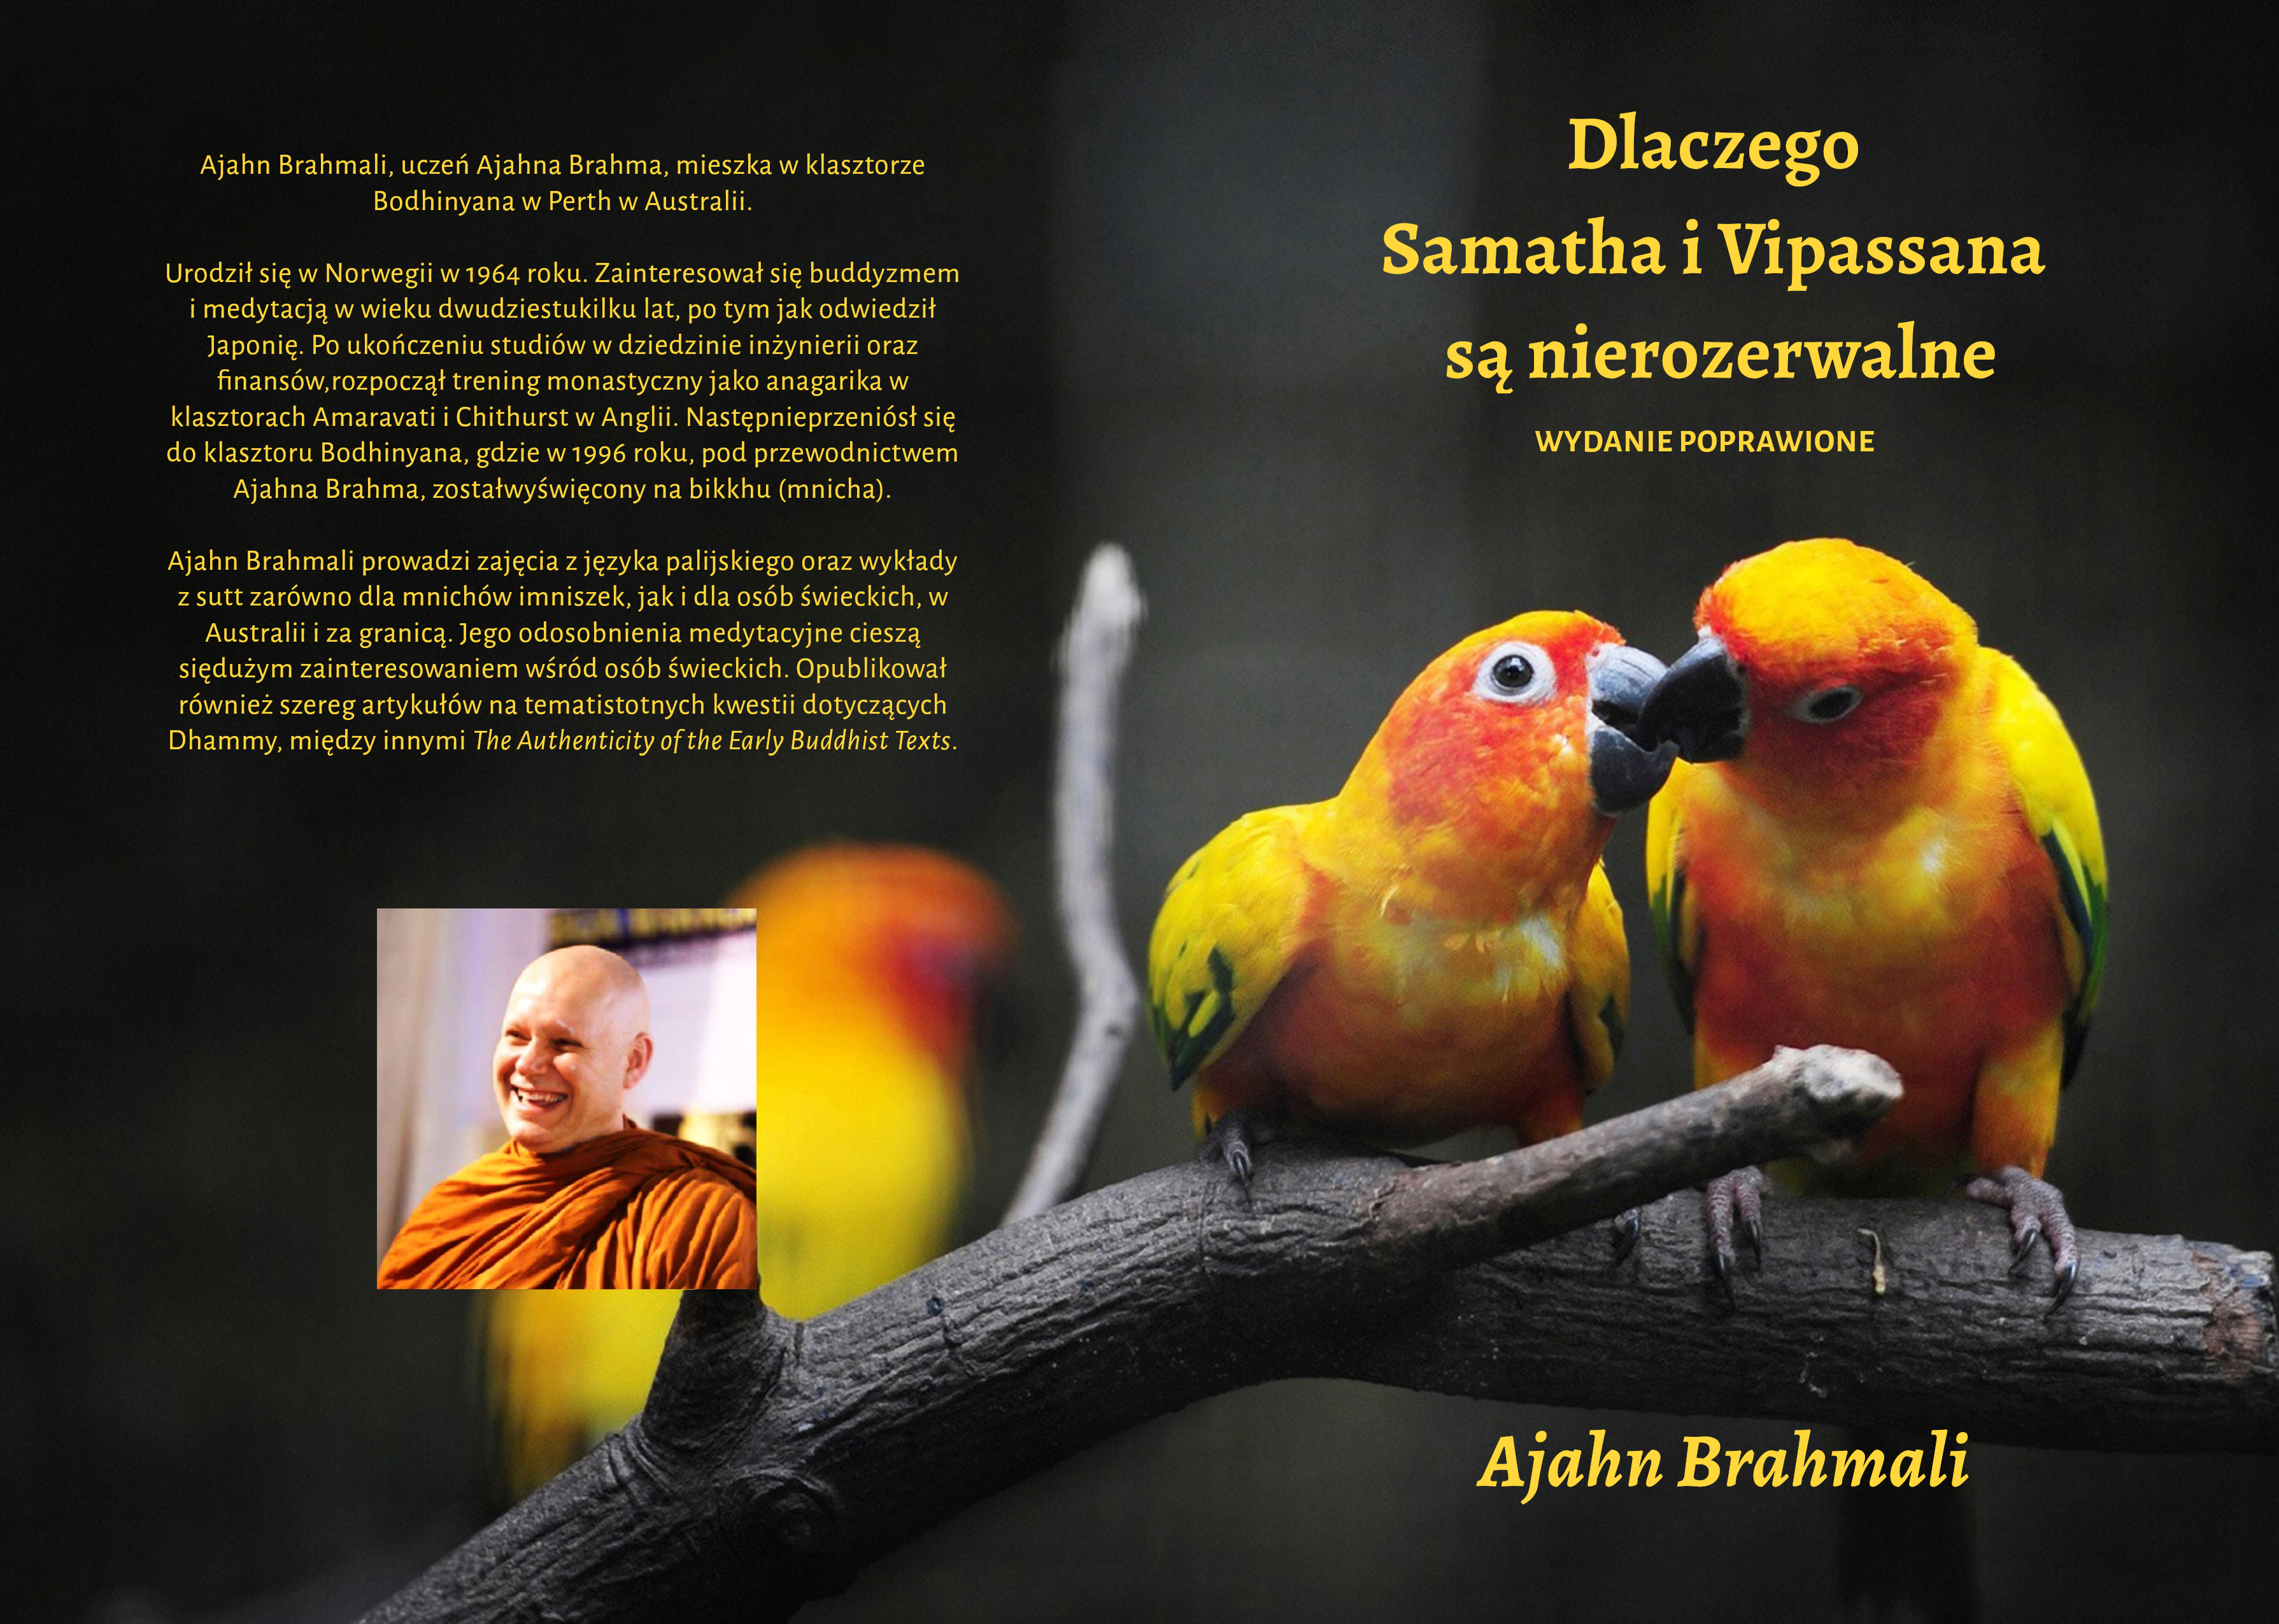
\includegraphics{sv-2_a5_cover}

\end{document}

